%!TEX root = ../template.tex
%%%%%%%%%%%%%%%%%%%%%%%%%%%%%%%%%%%%%%%%%%%%%%%%%%%%%%%%%%%%%%%%%%%%
%% chapter5.tex
%% NOVA thesis document file
%%
%% Chapter with lots of dummy text
%%%%%%%%%%%%%%%%%%%%%%%%%%%%%%%%%%%%%%%%%%%%%%%%%%%%%%%%%%%%%%%%%%%%

\typeout{NT FILE chapter5.tex}%

\chapter{System Design and Realization}
\label{cha:impl}


\epigraph{ \textit{This chapter describes the technical implementation of the proposed configuration language for RAMSES. It details how the insights from industrial collaboration informed the architectural decisions and how each feature was implemented.}}


\section{Industry Partner Meeting}
\label{sec:industry_meeting}

The first meeting with an industry partner revealed to be very useful with many insights to note, particularly that a few features were highlighted and prioritized in order to maintain a good development speed and an overall better plan. Most of the previously thought of features (\Glspl{identifier}, Traceability, Report, etc) were endorsed, however, a new feature was suggested by an expert \gls{ROS} developer: the separation of \gls{ROS} specific code and C++ specific code, meaning that code that is specific to \gls{ROS} can be isolated as it is very similar along the various generated files. This will essentially be done with an interface that will implement \gls{ROS} code on C++ only files, which effectively serves as a separation of concerns.

\begin{tcolorbox}[colback=green!5, colframe=green!40!black] This meeting provided extremely valuable insight as the industry partner has been using \gls{ROS} for over seven years, effectively distilling their experience into actionable knowledge. \end{tcolorbox}


\section{Implementation Plan} 
\label{sec:impl_plan}

In order to better understand what features will be implemented, when and why, the implementation will be done by layers, each layers will depend on things done previously on other layers, hence some features are developed before others.

\bgroup
\rowcolors{1}{}{GhostWhite}
\begin{xltabular}{\textwidth}{X X X}
	\caption{Feature dependency table}
	\label{tab:impl_plan}\\
	\toprule
	\rowcolor{Gainsboro}%
	Feature & Depends On & Notes \\
	\midrule
	\Glspl{identifier} & – & Core to code structure \\
	Comments & \Glspl{identifier} & Cheap to implement early \\
	Traceability & \Glspl{identifier}, Comments & Hard to retrofit later \\
	Report & Traceability & Uses trace data \\
	Standard\par Compliance & Report, Traceability & Enforce compliance early \\
	Dead Code\par Elimination & Traceability, Report & Needs stable generation logic \\
	Memory\par Optimization & Dead Code Elim, Traceability & Impacts data structures directly \\
	Node Interface & Memory Optimization & Enables \gls{ROS} decoupling \\
	File Management & Node Interface & Facilitates file management operations \\
	Legacy Code\par Integration & Node Interface & Most architecture-dependent \\
	\bottomrule
\end{xltabular}


Table~\ref{tab:impl_plan} presents the planned order of feature implementation based on their dependencies. Each feature may require elements developed in previous steps, ensuring a coherent and manageable progression. This dependency structure prevents rework by implementing features that provide necessary infrastructure before higher-level functionalities.


\subsection{Core and Metadata Layer}
\label{sec:code_and_meta}

The Core and Metadata Layer (Table~\ref{tab:core_and_meta}) includes foundational features that establish the basic code structure and metadata necessary for subsequent processing. Features such as \glspl{identifier} and comments form the backbone of the generator, while traceability and reporting provide essential tools for debugging and verification. Their relatively low to medium complexity allows them to be developed early, enabling smooth integration of more advanced features later.

\bgroup
\rowcolors{1}{}{GhostWhite}
\begin{xltabular}{\textwidth}{X X X}
	\caption{Core and Metadata features and their complexity}
	\label{tab:core_and_meta}\\
	\toprule
	\rowcolor{Gainsboro}%
	Feature   & Complexity  & Notes \\
	\midrule
	\Glspl{identifier} & Low & Nearly complete. \\
	Comments & Very Low & Can parallel \gls{identifier} completion. \\
	Traceability & Medium & Requires structured tagging throughout the generator. \\
	Report & Low-Medium & Build once traceability is present; not deeply complex. \\
	\bottomrule
\end{xltabular}


This first layer will serve as a base for other features to come since it has fairly straightforward but very useful features.


\subsection{Structural Optimization Layer}
\label{sec:struct_opt_layer}

The Structural Optimization Layer (Table~\ref{tab:struct_opt_layer}) focuses on improving code quality and efficiency. Standard compliance ensures generated code meets coding norms and best practices. Dead code elimination and memory optimization reduce code bloat and resource consumption but require stable metadata and analysis frameworks built in previous layers. These features have higher complexity, reflecting the need for careful analysis and manipulation of generated code.

\bgroup
\rowcolors{1}{}{GhostWhite}
\begin{xltabular}{\textwidth}{X X X}
	\caption{Structural Optimization Layer}
	\label{tab:struct_opt_layer}\\
	\toprule
	\rowcolor{Gainsboro}%
	Feature & Depends On & Notes \\
	\midrule
	Standard Compliance & Report, Traceability & Defining and checking rules\par requires steady effort. \\
	Dead Code Elimination & Traceability, Report & Non-trivial static analysis\par in model-to-code context. \\
	Memory Optimization & Dead Code Elim, Traceability & Impacts core data structure generation.\par Error-prone. \\
	\bottomrule
\end{xltabular}

The structural layer cements what was done before and adds to it with an optimization focused approach.

\subsection{Architecture Layer}
\label{sec:arch_layer}

The Architecture Layer (Table~\ref{tab:arch_layer}) introduces features that abstract and modularize the generated code to support scalability and maintainability. The node interface abstraction separates platform-specific code (\gls{ROS} dependencies) from core logic, facilitating reuse and easier updates. File management is a quality of life feature which is very sensitive as file naming and location must be consistent at all times. Legacy code integration is the most complex and architecture-dependent feature, involving interfacing with existing external codebases, which requires careful design and planning to avoid integration pitfalls.

\bgroup
\rowcolors{1}{}{GhostWhite}
\begin{xltabular}{\textwidth}{X X X}
\caption{Architecture Layer}
\label{tab:arch_layer}\\
\toprule
\rowcolor{Gainsboro}%
Feature & Depends On & Notes \\
\midrule
Node Interface & Memory Optimization & Architecture-dependent.\par Needs careful planning. \\
File Management & Node Interface & Affects every file directly \\
Legacy Code Integration & Node Interface & Undefined scope and\par likely the most architecture-sensitive \\
\bottomrule
\end{xltabular}

The last layer of implementation has a higher degree of abstraction and requires a much more project architecture understanding than the previous layers, which is why it is done last and after every other feature layer is implemented. This will allow for the full focus to be on these core features that will have a much higher individual impact on code generation than the previous ones.

\section{Implementation}
\label{sec:implementation}


As the implementation methodology was done iteratively and following the plan discussed in Section~\ref{sec:impl_plan}, the first feature to implement was the naming conventions.

\subsection{Naming Conventions}
\label{sec:impl_name_conv}

The implementation of naming conventions was straight forward since the demo developed in Section~\ref{sec:proof_of_concept} was a pretty big portion of the whole thing. Using Acceleo we are able to modify the properties coming from the model as they are added into the C++ file, in this case, the name is formatted according to the selected convention. The main addition to the prototype work was the introduction of dynamic naming conventions that depend on the selected language, for example: in C++, classes are declared in PascalCase, whereas variables are declared in snake\_case, the following generated code illustrates that very well:

\begin{verbatim}
	class ImageDisplay : public rclcpp::Node
{
	public:
	
	ImageDisplay(): Node("ImageDisplay")
	{
		
		image_subscriber_sub_ = this->create_subscription(...);
		
		nd_spinner_sub_ = this->create_subscription(...)
\end{verbatim}

As we can see, ImageDisplay and image\_subscriber\_sub\_ are both \glspl{identifier} but each one has a different format. In contrast, the previous implementation without configuration was strictly be \textit{Image\_Display} and \textit{Image\_Subscriber\_Sub\_}. These names come directly from the \gls{AADL} model as \textbf{\textit{Image\_Display} and \textit{Image\_Subscriber}}.

To summarize, the whole naming convention implementation consisted in:

\begin{itemize} 
	\item The ability to change \gls{identifier} (class, variable, method) formats dynamically from a list of implemented options (camelCase, UPPERCASE, lowercase, snake\_case and UPPER\_SNAKE\_CASE).
	\item Based on the selected language, assign different styles to different \glspl{identifier}.
	\item Option to input a prefix or suffix in every \gls{identifier}\footnote{This affix is not affected by the naming convention.}.
\end{itemize}

This implementation was very important since the remaining features used it to the fullest, hence why it needed to be the first.


\subsection{Comments}
\label{sec:impl_comments}

The implementation of dynamic code comments allow the user to get much more context on the code while preserving the ability to view raw, non-commented code. The way it works is pretty straight forward, the user can toggle the comments on or off, comments are dynamic according to their component and only provide essential info.

\begin{figure}[htbp]
	\centering
	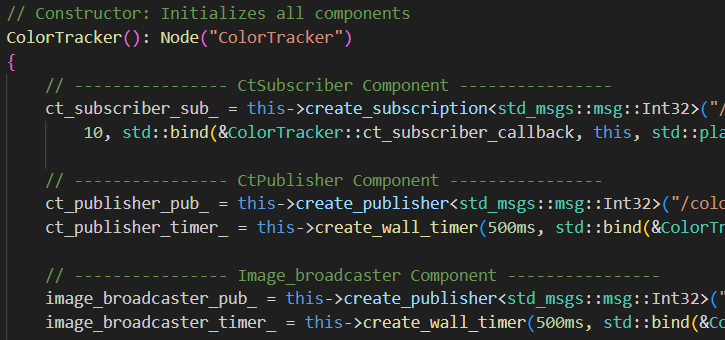
\includegraphics[width=\textwidth]{comments.png}
	\caption{Example of generated code with comments}
	\label{fig:comment}
\end{figure}

Figure~\ref{fig:comment} illustrates how the comments vary depending on the component, this also provides a degree of separation that helps developers understand where parts of the input model are being implemented.

More examples of code comments (with before and after) can be found in the Appendix~\ref{app:comment}.

In addition to this, there is also the possibility to display a Copyright Notice in the first lines of every file along with an author reference. This small detail is a best practice that aligns with industry standards and serves multiple practical purposes such as clarifying ownership of the code, preventing copyright infringement and overall maintaining professionalism.


\subsection{Traceability}
\label{sec:impl_trace}

The implementation of traceability is related with the report feature, however, traceability can exist without a report and a report can exist without traceability~\ref{sec:impl_report}. The main idea of traceability is to relate the coding files directly to the model so we are able to verify that a certain file came from a certain part of the model.

The base construction of the trace file was done in JSON, this provides information while still maintaining a structure that can easily be ported elsewhere.

This is an example of the JSON produced by a traceability analysis:

\begin{verbatim}
{
	"system": "Robot_Vision_I_Instance",
	"generatedAt": "2025-07-28 16:26:49",
	"location": "C:/Users/aurel/git/codegen-config/fr.mem4csd.codegen.config/results",
	"components": {
		"Usb_Cam_Nd": {
			"file": "robot_vision_i_instance/src/Usb_Cam_Nd_process.cpp",
			"type": "process",
			"subcomponent": [
			{
				"name": "Image_Broadcaster",
				"qualifiedName": "Robot_Vision_I_Instance::Usb_Cam_Nd::Image_Broadcaster",
				"codeTrace": "@trace name='Image_Broadcaster'",
				"line": "15",
				"type": "thread",
				"properties": {
					"Dispatch_Protocol": "",
					"Period": ""
				}
			},
			{
				"name": "UsbSpinner",
				"qualifiedName": "Robot_Vision_I_Instance::Usb_Cam_Nd::UsbSpinner",
				"codeTrace": "@trace name='UsbSpinner'",
				"line" : "20",
				"type": "thread",
				"properties": {
					"Dispatch_Protocol": "",
					"Period": ""
				}
			}
			]
		},(...)
\end{verbatim}

As we can see, it relates the model to the code in various forms, mainly code traces, qualified names, file and package locations. On top of that, it provides additional info that is useful for both developers and end users, developers can easily use this \gls{JSON} as input for various tools (generating an alternate report from the one provided for example) and users can use it to trace parts of the code dedicated to a specific component or subcomponent using a combination of the file locations, code traces and line number.

The way the line number is detected is quite complex in practice but more straightforward in theory:

\begin{itemize} 
	\item When traceability is enabled, the code generates with traces, those traces are not language or tool specific, hence they don't get picked up by other tools or as language syntax.
	\item The same traces are generated in the \gls{JSON}.
	\item Using the \gls{JSON} and the traces corresponding to sub components in the larger component (which is represented by a C++ file) the C++ files are scavenged for traces, which, when found, get saved directly below the \textit{codeTrace}, as the line correspondent to it.
\end{itemize}

In addition to this, traceability links were created using Capra to ensure that the \gls{JSON} file can be directly related to the C++ files using the \textit{@trace} indicative.

\subsection{Report}
\label{sec:impl_report}

The report was implemented with the goal of providing a clear, concise and structured way of visualizing exactly how the model translates to code. To do this, the report is generated in \gls{HTML} using Acceleo. This is important since it overcomes a few constraints, mainly:

\begin{itemize} 
	\item \textbf{PDF with Java:} The major issue that producing \gls{HTML} code with Acceleo instead of a direct PDF with Java fixes is that producing PDFs with Java code, although more practical on the surface, has many limitations when it comes to designing and structuring PDFs. In addition, the verbose is very unintuitive and can quickly grow in complexity.
	\item \textbf{Extensibility:} Since \gls{HTML} is a simple and well known language, adding details and making changes is straightforward when comparing it to other tools like LaTeX. In this case, the usage of LaTeX isn't really justified since it is more directed to academic circumstances and not fast paced development. 
	\item \textbf{Styling Issues:} Using raw \gls{CSS} in combination with \gls{HTML} is no doubt the best choice when it comes to styling the report. Java has many limitations when it comes to styling and LaTeX is very strict and error prone. For a basic report such as the one generated, \gls{CSS} styling is more than enough.
\end{itemize}

Once these constraints were no longer an issue, the development of the report was much more intuitive. The base was made with \gls{HTML} and \gls{CSS}, which enabled a high degree of custom styles while also simplifying the integration of useful information. 

Since the first iteration of the report was done in \gls{HTML}, the transition to PDF was mostly seamless, however, its implementation was done not by Java code, but via Workflow. This was at a later stage, a more detailed explanation can be found in Section~\ref{sec:workflows}.

The report has many features, its high customization enables the creation of different parts when needed, hence omitting redundant or unwanted sections according to user needs. One of the core elements is the \gls{ROS} specific option, which highlights \gls{ROS} specific components that were generated or ported from the model. This allows \gls{ROS} developers to have a much clearer idea of how parts of the input model were represented in the \gls{ROS} part of the code, for instance, what thread corresponds to a Publisher\footnote{Publishers generate and publish data (sensor readings, etc).} or Subscriber\footnote{Subscribers listen for and process data sent by Publishers.}.

\subsection{Code Quality Checker}
\label{sec:impl_code_qual_checker}

A fine addition to the code generator was the introduction of a code quality checker powered by \textit{Cppcheck}, which analyses every generated code file an points out errors immediately after generation. This allows the end user to quickly identify syntax errors and common code problems\footnote{This certainty is based on the capability that \textit{Cppcheck} has to report code errors. It does not guarantee that the code is semantically functional, just syntactically correct.}

Moreover, the code can be analyses at any point, meaning that \textit{Cppcheck} can verify the correctness of user generated code if needed. Providing value even after being used for its main purpose.

\subsubsection{Cppcheck}
\label{sec:impl_side_cppchecker}

\textit{Cppcheck} is a static analysis tool for C and C++ code, it's designed to detect a wide range of programming errors, potential bugs, and code style issues without executing the program. \textit{Cppcheck} analyzes the source code to identify problems such as memory leaks, uninitialized variables, unused functions, and violations of coding best practices. It's a lightweight, platform-independent, and highly configurable tool, which makes it suitable for integration into our code generation workflow.

\textit{Cppcheck} has both an open source and a commercial version, in this case, 

\subsection{ROS and C++ separation}
\label{sec:impl_ros_separation}

One of the underlining problems of the base generated code was the fact that \gls{ROS} code and C++ code where closely coupled together. This is an issue since most of the C++ implementation is \gls{ROS} independent, meaning that it could, in theory, be reused in contexts where \gls{ROS} is not available or not needed. However, since the generated code is tight coupled with \gls{ROS}, it forces the presence of ROS-specific dependencies even in parts of the system that do not require them. 

To combat this, a new approach to code generation was implemented. The main goal was to port the \gls{ROS} code inside the C++ files onto another folder, adjacent to the remaining C++ files. This can be better understood visually, we part from this:

\begin{verbatim}
src/
	 Color_Tracker_process.cpp
	 Image_Display_2_process.cpp
\end{verbatim}


And we split the files into their \gls{ROS} and C++ counterparts, like so:

\begin{verbatim}
src/
	 impl/
		 Color_Tracker_logic.cpp
		 Image_Display_2_logic.cpp
	 ros/
		 Color_Tracker_node.cpp
		 Image_Display_2_node.cpp
\end{verbatim}

With the files now separated, it is possible to reuse the C++ code present in the impl folder without the \gls{ROS} dependencies. This also opens more the window to the inclusion of company specific libraries that can, if needed, be split into \gls{ROS} and C++ only counterparts.

To further improve on the \gls{ROS} side of the customization, there is also the option to choose the thread executor for the given node\footnote{This also takes effect when decoupling is disabled.}. There are three fundamental thread executors, they can be described as follows:

\begin{itemize} 
	\item The Single Threaded Executor processes all callbacks (from incoming messages, timers, services, and events) of one or more nodes in a single thread, ensuring that only one callback executes at a time.
	\item The Multi-Threaded Executor creates a configurable number of threads to allow for processing multiple messages or events in parallel.
	\item  The Static Single-Threaded Executor optimizes the runtime costs for scanning the structure of a node in terms of subscriptions, timers, service servers, action servers, etc. It performs this scan only once when the node is added, while the other two executors regularly scan for such changes. 
\end{itemize}

These three options fundamentally do not change how the generated runtime application works, but they give it different options when it comes to managing execution performance.

\begin{tcolorbox}[colback=blue!5, colframe=blue!40!black] Some complex applications might benefit from multi-threading while more simple ones can offer the fairly same performance in any threading type.
\end{tcolorbox}


\subsection{File Management}
\label{sec:impl_file_mng}

The intent of having a file management option in the configuration was to dynamically manage how the files are generated, including if they overwrite previously generated files.

The main addition however was the ability to add a header prefix to every generated code file, further facilitating copyright and licensing enforcement.

This file header can be any phrase or character but due to operating system restrictions, some character have to be filtered out, here is an example of this filtration:

\begin{verbatim}
  ..CON:my*file?<>|aux\0COM1  "

			↓

CON_my_file____aux_0COM1___
\end{verbatim}

By default, any forbidden character is replaced by an underline and spaces at the start and end of the word are trimmed. This eliminates eventual errors in the code execution.

A good example of the result of this file header implementation is, based of the files in Section~\ref{sec:impl_ros_separation}, when adding the header \textit{Nova"} becomes:

\begin{verbatim}
	src/
		 impl/
			 Nova_Color_Tracker_logic.cpp
			 Nova_Image_Display_2_logic.cpp
		 ros/
			 Nova_Color_Tracker_node.cpp
			 Nova_Image_Display_2_node.cpp
\end{verbatim}

Note that the apostrophe is transformed into an underline as mentioned previously.

The overriding system is another file management option. Previously, the code generator simply generated the files in any circumstance, effectively replacing every file, every time. In a simple model this is not an issue, however, in a larger model this can quickly become a performance bottleneck since it implies generating everything, every time. 

When overriding is enabled, the generator does not change, it still generates every file every time, when it is disabled however, it only generates files that are not yet present. For instance, if we have a complete project, no new files will be generated or substituted, in contrast, if one file is missing, the generator will generate only the missing file.

Even preliminary tests produced a significant difference in execution time when overriding is disabled\footnote{Up to 500ms less than the override enabled counterpart.}, proving that it is worth it to give the user the choice between generating the whole project or just specific parts of it.

\subsection{Legacy Code Integration}
\label{sec:impl_legacy_code}

The main problem that legacy code integration solves is the following:

There are C++ libraries that need to be used by specific \gls{ROS} components, these libraries should be included in the \gls{ROS} project when needed.

To put it simply, in order to produce the functionality that the input model entices, certain legacy libraries need to be included, not just in the project, but called in the code aswell. The way it was done is clear:

\begin{itemize} 
	\item Firstly, libraries that the code will need based on model components used are listed.
	\item Then, the code for those libraries is copied to the project folder.
	\item Lastly, this newly copied code is called in certain places based on functional necessity.
\end{itemize}

\subsection{Generation Hooks}
\label{sec:impl_gen_hooks}

The need to run certain scripts before or after project execution is very valuable. Either being quick cleanup scripts to prepare the project folder for a new version or post generation scripts to automatically test the generated project, these scripts can bring value and a higher of automation to any project.

For those reasons, generation hooks where included in the configuration language. The premise is fairly simple: to execute user created code before or after the actual code generation.

Even though that option is available in the configuration, in the specific case of \gls{RAMSES}, there is no need to define a component that executes a script, meaning that there is already a way to execute terminal based commands in the project. The definition was still kept in the configuration language although it was not implemented in practice due to a more practical option that is depicted in Section~\ref{sec:workflows_script_executor}.

************** TODO: Describe generation hooks applied in testing

\subsection{Multiple Configurations}
\label{sec:impl_multi_config}

When testing the previously finished features, a few issues stood out: 

\begin{itemize} 
	\item The difficulty to quickly change from one configuration to the other.
	\item Handling multiple configurations at the same time.
\end{itemize}

The main problem is that, if we want to create and customize a new configuration we have to start from scratch and use a new file. To combat this issue, a new way of creating configurations was introduced: the list of configurations.

The premise is that instead of having multiple files, each one representing a different coding language, there is a single file with a list of configurations.

\begin{figure}[h]
	\centering
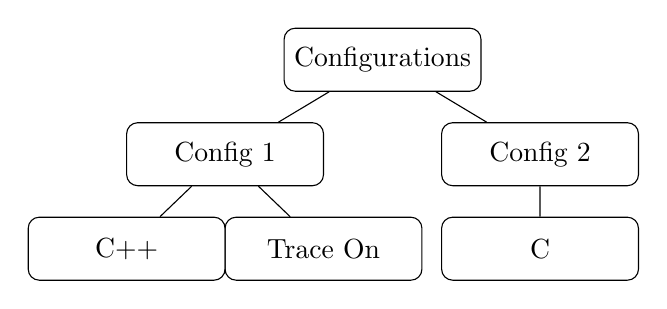
\begin{tikzpicture}[
	level distance=12mm,
	level 1/.style={sibling distance=40mm}, % distance between Config 1 / Config 2
	level 2/.style={sibling distance=25mm},
	every node/.style={
		draw, rounded corners, align=center,
		minimum width=2.5cm, minimum height=8mm
	}
	]
	
	% Left tree: Configurations
	\node {Configurations}
	child {node {Config 1}
		child {node {C++}}
		child {node {Trace On}}
	}
	child {node {Config 2}
		child {node {C}}
	};
	
\end{tikzpicture}
\hspace{1cm}
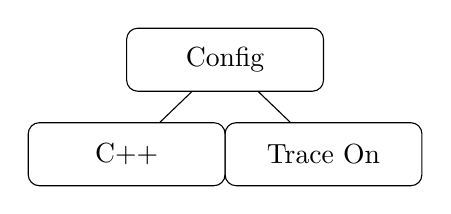
\begin{tikzpicture}[
	level distance=12mm,
	sibling distance=25mm,
	every node/.style={
		draw, rounded corners, align=center,
		minimum width=2.5cm, minimum height=8mm
	}
	]
	
	% Right tree: Single Configuration
	\node {Config}
	child {node {C++}}
	child {node {Trace On}};
	
\end{tikzpicture}
\caption{Comparison between multiple configurations (left) and a single configuration (right).}
\label{fig:tree_config_comparison}
\end{figure}


This way, instead of handling multiple files we can, like illustrated in Figure~\ref{fig:tree_config_comparison}, manage every single configuration in one file and the same configuration can be used by different generators since each one can find the configuration it needs.

This is an addition, not a restriction, so, as we will explore more in the next section~\ref{sec:workflows}, we can still use a single configuration as input or a list of configurations, further improving the flexibility of the code generator.


\section{Workflows}
\label{sec:workflows}

The process of generating files involves feeding both a configuration and input model to the generator, which then processes this into C++ code, an \gls{HTML} report or a traceability \gls{JSON}. There are many issues that arise from the way the generation process works, mainly that:

\begin{itemize} 
	\item Many Java main classes have to exist.
	\item In order to generate everything needed to run a \gls{ROS} project many Java methods have to be run.
	\item These methods cannot be run in a single click, as that would require a complete redesign of the current architecture.
\end{itemize}


The solution for this are workflows. Workflows allows the automation of certain tasks, e.g., reading, writing, or transforming models, by plugging together several workflow components, which are executed consecutively. A workflow component performs a certain task and can be configured with parameters.

This allows for the execution of specific parts of the code generation in an isolated way, as well as the execution of every part needed to produce a complete and functional \gls{ROS} project, on top of that, \gls{JUnit} tests based on workflows are also possible and already a common pattern on the \gls{RAMSES} project.

\subsection{Acceleo Workflow Component}
\label{sec:workflows_acceleo}

The custom workflow component created was the AcceleoGeneratorComponent, which simply parsed all the inputs (AADL input model, configuration and output folder) and executed the Java class responsible for the specific code generation.

The beauty of this component is that it is optimized to every single Acceleo Java class present in \gls{RAMSES}, meaning that, in the workflow, every Java class can be represented by a AcceleoGeneratorComponent which facilitates the sequential execution and removes the need to have components specific to a certain class.

In a similar fashion, changing the inputs of the generation is also much simpler than before as there is a property for each of those (\gls{AADL} model, configuration model, working directory and output folder) in the workflow, facilitating the change in the AcceleoGeneratorComponents: a simple change to the property will affect all the workflow components that use that property.


\subsection{Dynamic Acceleo Workflow Executor}
\label{sec:workflows_dynamic_executor}

The custom component described in the previous Section~\ref{sec:workflows_acceleo} works flawlessly for its main purpose, however, a key issue arose: instead of feeding the template to the model, we feed the class that that template represents. This is an issue since if we want to execute a specific Acceleo template we need its class.

The solution to this problem was clear: instead of calling the classes independently, the component would call a generic class that would handle any Acceleo template. This did not come without drawbacks, mainly that handling every template the same way reduced their overall specialty. This was an issue that the previous component solved by integrating additional functionality in each individual class as needed.

Essentially the two architecture choices where either full specialization but low integration capabilities or high integration and low specialization. However, the third option was both.

A new version of the Acceleo custom Workflow component was devised, the premise was that the component would receive the template name (not the class name) and search for the class represented by the given component, if none was found the component would fallback to the generic Acceleo generator class. This hybrid architecture means that, when feeding a template name that does not have a Java class associated, the Workflow will execute it seamlessly, provided it has an \gls{AADL} model and a configuration file. Similarly, if there is the need for a more in depth execution, a Java implementation of the template can still be done.


\subsection{Script Workflow Executor}
\label{sec:workflows_script_executor}

One of the features mentioned both in the feature model~\ref{label} and in the client meeting~\ref{label} was the ability to execute pre or post generation hooks as discussed in Section~\ref{sec:impl_gen_hooks}. 

This functionality was primarily aimed to be present in the \gls{DSL} as a way to execute Java code to consequently run a command script, however, in the very specific case of the \gls{RAMSES} environment, a different option is more viable and already implemented: System Command Component.

The System Command Components allows for the execution of commands in a terminal (in this case a Windows terminal) by passing values in its Workflow component properties.

When running a script before code generation occurs, we need the following:

\begin{itemize} 
	\item \textbf{Arguments: } $\backslash$c, pregen.bat\footnote{This represents executable that we want to run.}
	\item \textbf{Command: } cmd
	\item \textbf{Working Directory: } file:/C:/Users/user/robot\_vision\_i\_instance
\end{itemize}

With this information, the SystemCommandComponent runs a terminal on the given directory that executes the command \textit{cmd $\backslash$c pregen.bat}, effectively executing the file \textit{pregen.bat}.


\subsection{Execution Times}
\label{sec:exec_times}

With the workflow built and running, it was possible to get an idea of the execution times of each part of the workflow.

\subsubsection{First Workflow Execution Time Test}
\label{sec:exec_times_v1}

To perform the first volley of workflow execution time tests, a functional \gls{AADL} model was picked due to its correctness and previous usage in some examples. The configuration was also tuned to its maxed settings, meaning that every option was checked (report generation, traceability, etc) so that it would produce a better range of timetables, the complete configuration details for the this context can be found in~\ref{app:config_first_batch}.

In this phase, 15 execution runs where documented, which can be found in the Appendix~\ref{tab:workflow_exec_times_1}.

\begin{figure}[htbp]
	\centering
	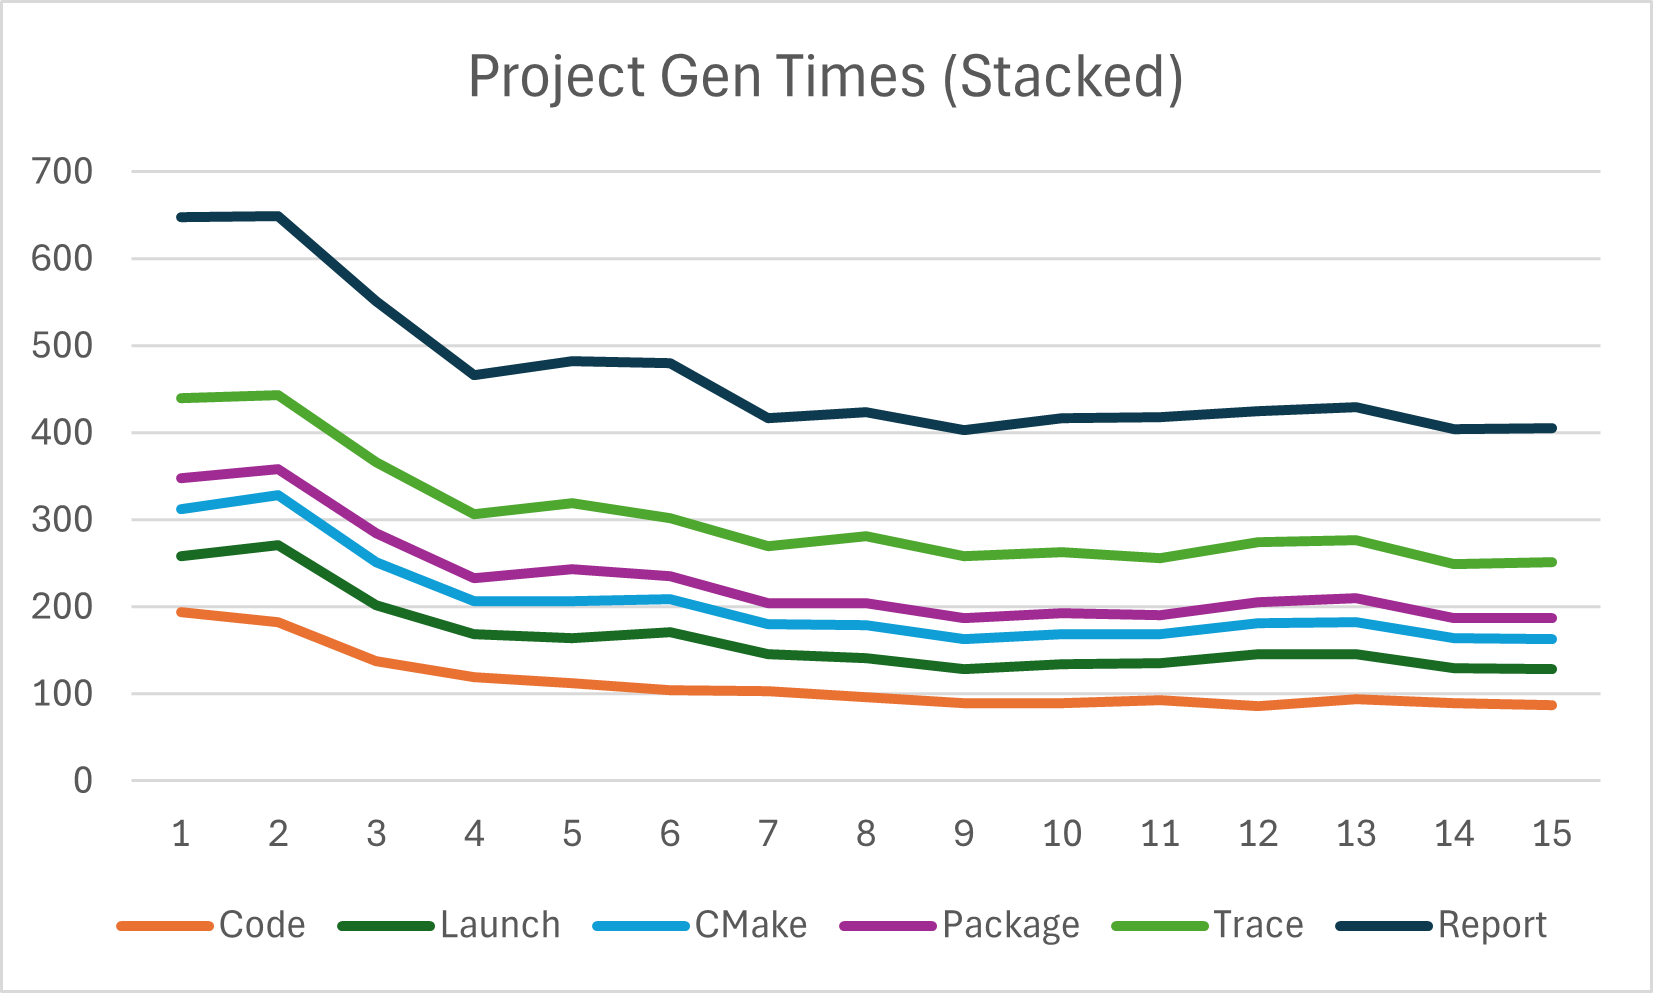
\includegraphics[width=\textwidth]{exec_times1.png}
	\caption{Code generation execution times}
	\label{fig:exec_times_1}
\end{figure}

Taking a look at Figure~\ref{fig:exec_times_1} we can see that naturally some parts of the workflow take more time than others, mainly the code generation and the report generation.

The Launch, CMake and Package files take much less time than the other ones due to their simplicity and to the fact that they generate a single file, as opposed to the Code generation which, in this case, generates 7 C++ code files. The report takes even longer than that because, on top of documenting the generated files and build an HTML report, it also checks those files for code quality issues, which ends up taking even more time. The JSON Trace file is pretty straightforward, however, since it scavenges the code files for the exact placement of the traces, it does end up with an execution time bigger than the other single file generations.

Since the base project did not have a workflow that successfully implemented the ancient Java code, it is not possible to directly compare the execution times of the old version of the code generation with the new one. However, we can estimate the time it took to execute a project generation in the ancient generator with the information from Table~\ref{app:workflow_exec_time}, which, after measuring the time it takes to generate the Launch, CMake, Package and C++ files, comes around to 231,6ms, essentially half of the current average execution time of 479,9ms. This is expected since both the Trace and the Report take a significant amount of time. This interval can be even bigger if we consider that the original code generator did not even have a configuration file.

\begin{figure}[htbp]
	\centering
	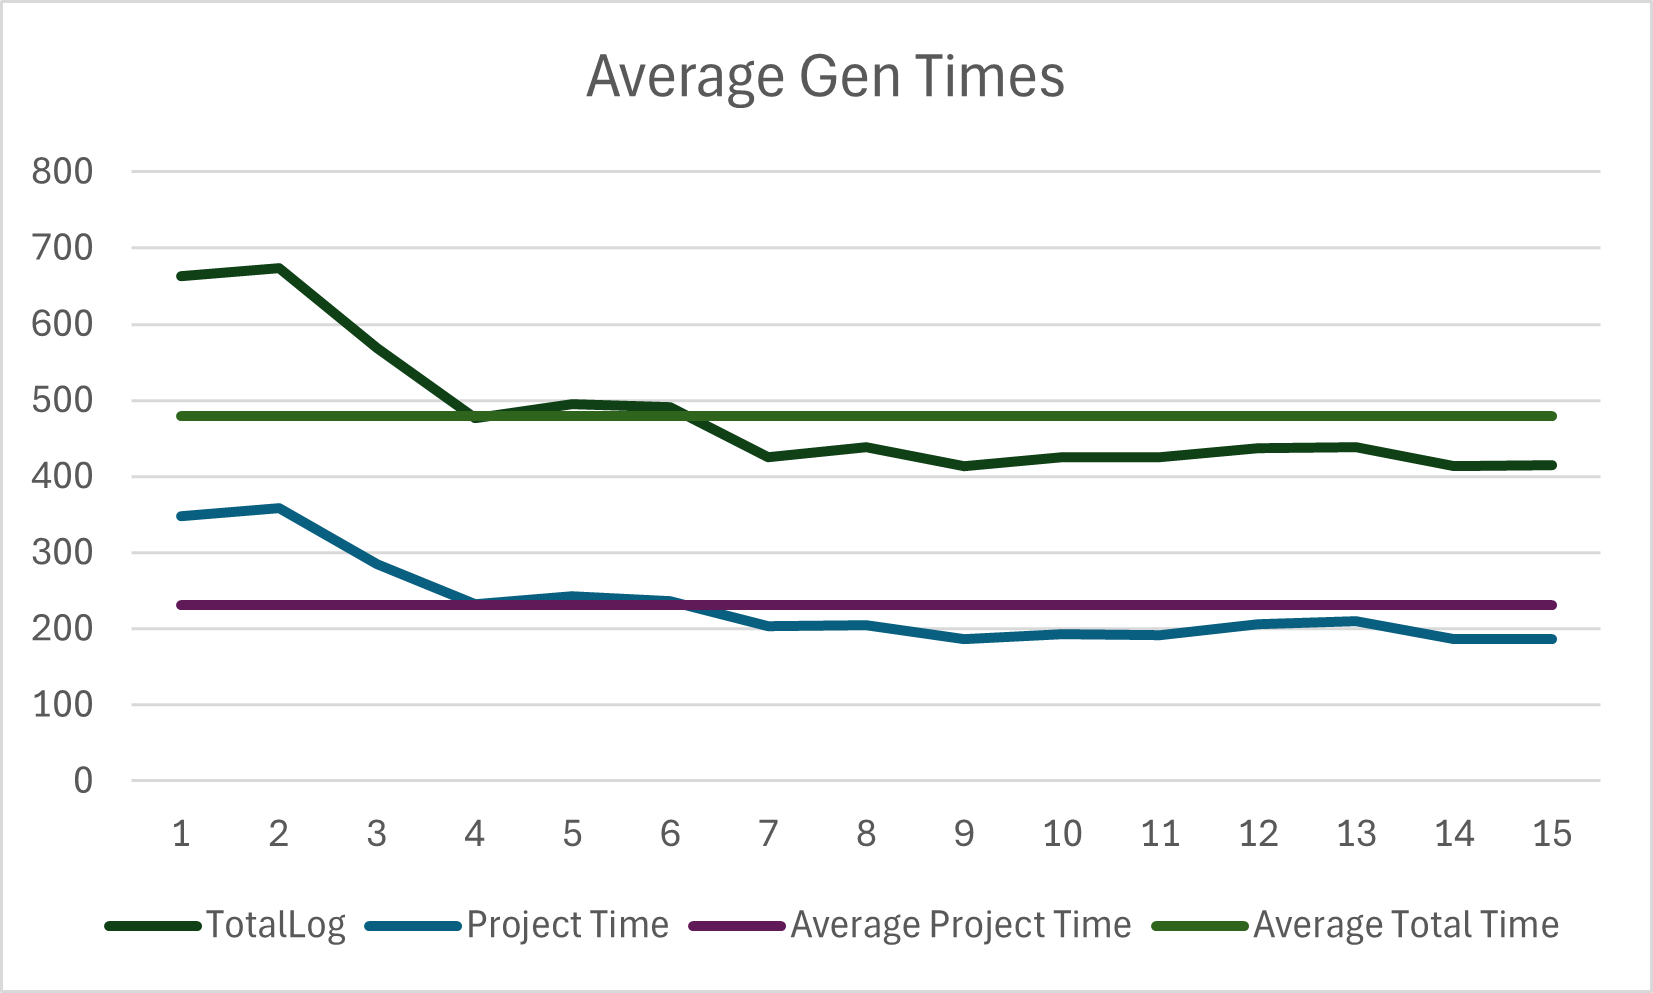
\includegraphics[width=\textwidth]{avg_exec_times_1.png}
	\caption{Average code generation execution times}
	\label{fig:avg_exec_times_1}
\end{figure}

As mentioned previously, Figure~\ref{fig:avg_exec_times_1} confirms that the average execution time seems to have doubled with the introduction of more processing heavy modules (Trace and Report), this is not a big issue as the total execution time is still below 500ms which is still very acceptable for the current conditions.




\section{Domain Specific Language}
\label{sec:dsl}

In order to customize the output of \gls{RAMSES}'s code generation, a \gls{DSL} was created using the Ecore framework. Which enabled a clean and straightforward way of defining configuration options based on code generation needs.

The configuration language as a base can be used in two formats:

\begin{itemize}  
	\item \textbf{Single configuration: } Configuration that allows the selection of language, naming convention, report options, architecture choice, file management, code comment management, traceability options and generation hooks.
	\item \textbf{List of configurations: } Dynamic list of configurations that allow for quick change and assignment of configurations when used.
\end{itemize}


As specified in Section~\ref{sec:impl_multi_config}, this choice is highly beneficial since it provides more flexibility to the usage of the configuration language itself with no notable drawbacks.

Going more in depth, the \gls{DSL} offers specific options given each topic, notably:

\begin{itemize}  
	\item \textbf{Language\footnote{Currently only 2 options, will be expanded in the future.}: } C++ or C.
	\item \textbf{Naming Convention\footnote{Derived directly from Section~\ref{sec:example}}: } Style (UPPER\_CASE, lower\_case, etc), affix and affix position.
	\item \textbf{Report: } Generate (whether the report gets generated or not), include traceability, include summary tables, include logic summaries (in the case of \gls{RAMSES}, \gls{ROS} summaries), show detected errors and open automatically.
	\item \textbf{Business Logic: } Decouple (separate from the code) and executor choice (Single executor, multiple or single static executor).
	\item \textbf{Files: } Overwrite existing, output directory and header prefix.
	\item \textbf{Code comments: } Enable, copyright notice and author.
	\item \textbf{Traceability: } Enable and produce diagram.
	\item \textbf{Extension: } Pre and post generation scripts.
\end{itemize}

These options control each part of the generated project and together they offer a high degree of customization to the generated code. 

\subsection{Language}
\label{sec:dsl_lang}

The language option defines the targeted language for the current customization. Meaning that the rest of the options may act differently based on language. On top of that, the language also serves as a distinction between different configurations in the configuration list, allowing for the quicker identification of the selected language in the generation.

This option also serves to map the code \glspl{identifier} to their language specific casing\footnote{This only applies when the naming convention is set to STANDARD.} as explained in Section~\ref{sec:dsl_lang}.

This option is highly extensible and, as \gls{RAMSES} grows, can be extended with many other languages such as Java, Assembly, Kotlin, etc.

\subsection{Naming Convention}
\label{sec:dsl_name}

The essence of the naming convention option is simple: to automatically change the casing on \glspl{identifier}.

\subsubsection{Identifier Style}
\label{sec:dsl_name_style}

The format on the style is done by analyzing the selected option in the configuration and then applying the style that corresponds to that option before code generation takes place. On top of the code, this also applies to every other instance of that identifier (CMake files for example), ensuring that every reference to that \gls{identifier} still preserves the style.

Most styles simply change every \gls{identifier} to the same style, examples of this are \textit{snake\_case}, \textit{PascalCase}, \textit{camelCase} and many others. The \textit{DEFAULT} option leaves identifiers exactly as they have been written in the model, allowing for an effective nullification of the formatting process.

The \textit{STANDARD} naming convention differs from the others as it allows for a dynamic \gls{identifier} naming, for instance: it allows \textit{Classes} to be \textit{Pascal\_Case} while simultaneously having \textit{Variables} in \textit{snake\_case}. This is very useful for specific restrictions where languages need different casing based on \gls{identifier} (Classes, methods, variables, constants, etc). This specific casing is very configurable and can be adapted to different programming languages, further improving the adaptability of the \gls{DSL}.


\subsubsection{Identifier Affix}
\label{sec:dsl_name_affix}

To complement the previous formatting, we can also add specific text (an affix) to the start or end of all \glspl{identifier}, this, then again, preserves the functionality while also adding a layer of customization to the code that offers many benefits such as: ************* say benefits ***************

The affix is not affected by the style formatting.













